
``Remote Sensing'', simply defined as the observation of geographic features and phenomena from a distance, was first coined by Ms. Evelyn Pruitt in the early 1950s. Pruitt, a geographer in the U.S. Navy's Office of Navel Research, felt there was a need to assign a name to the field of study extensively used in World War II, due to the rapid advancement of the imaging capabilities of cameras and scanners at the time. Today, remote sensing is defined as the practice of deriving information about Earth's land and water surfaces using images acquired from an overhead perspective, generally satellites or aerial shots. This is done through the detection of electromagnetic radiation reflected and emitted from the Earth's surface and atmosphere \cite{campbell2011introduction}. 

%A few key events will be described in this report to trace back the roots of remote sensing. \cite{campbell2011introduction}

\subsection{A Brief History of Satellite Remote Sensing and Landsat}
In the early 1800s, photosensitive chemicals were proposed for use in experiments to capture images. Several decades later in 1839 the preliminary results of these investigations were publicly reported by one of the founding fathers of photography, Louis Daguerre. This date forms the convenient arbitrary milestone for the birth of photography. The first aerial photograph milestone has generally been accredited to Gaspard F\'elix Tournachon, in 1858 when he acquired an aerial photograph from a camera tethered to a balloon in France. Over the years, numerous improvements were made to photographic technology, balloons and kites \cite{campbell2011introduction}. 
\par
In World War I, cameras were placed on aeroplanes for reconnaissance. Then, during the height of Cold War, the U.S. Government developed imaging satellites using specialised photographic film. An example of this is the CORONA photo-satellite resonance system launched in 1960 due to the suspension of U-2 spy plane. Figure 1 shows main recognisance system of the CORONA after deployment \cite{CORONA}. 
\par



%Modern day remote sensing and satellite imaging goes beyond military or strategic applications. As of September 1$^{st}$ 2021, there are 4,550 known operational satellites of which 1030 are for Earth observation \cite{Sat_Data}. Satellite imaging has a major applications in a wide range of industries from monitoring crop growth to forecasting weather.
%This report will focus on cloud cover over Earth, weather forecasting and terrain identification. 


\begin{figure}[H]
\centering
%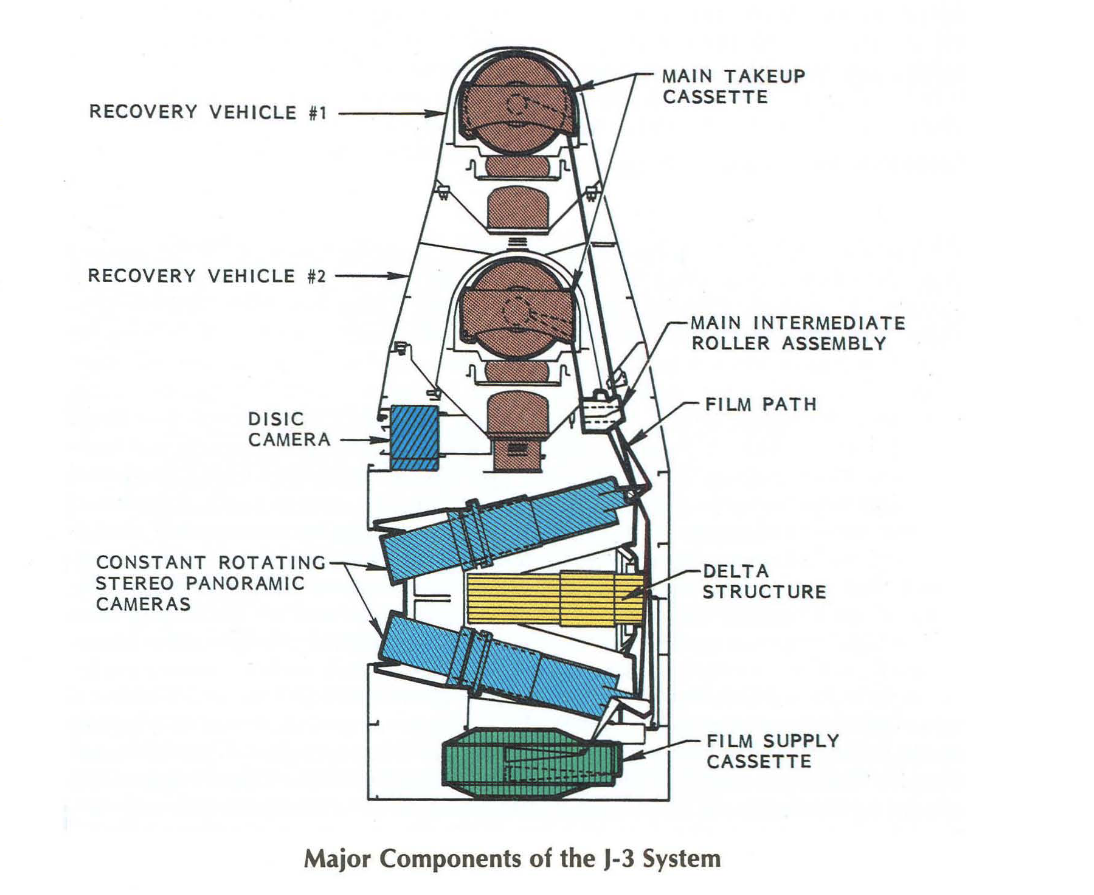
\includegraphics[totalheight=0.3\textheight]{j-3_system.png}
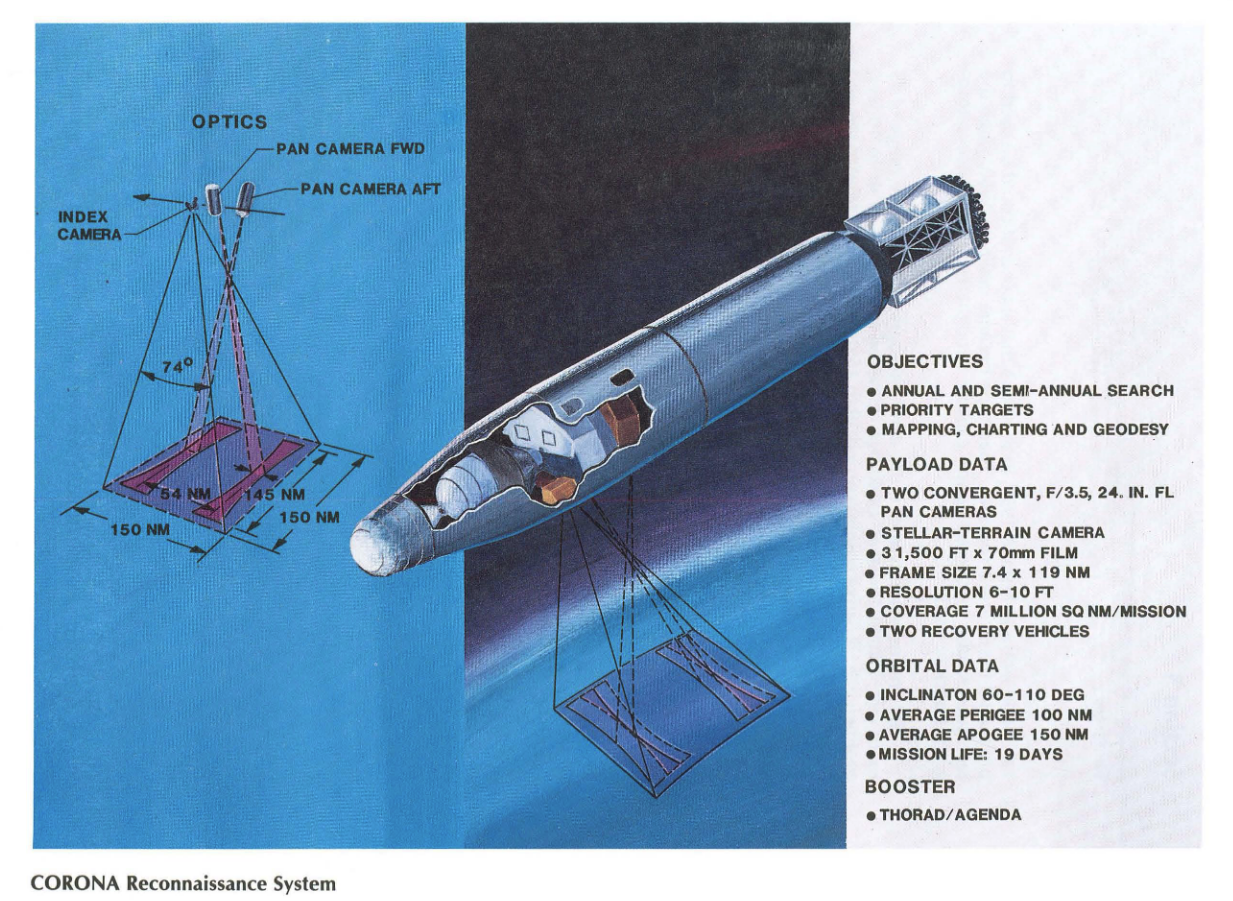
\includegraphics[totalheight=0.3\textheight]{CORONA REC .png}
\caption{CORONA Reconnaissance System's main objectives were to map, chart and survey areas of interest in enemy territories. The system is able to cover $\mathrm{2.4x10^{7}}$ km$^{2}$ per mission with a resolution of 2-3 meters \cite{CORONA}. The life of the mission is 19 days, after which the film rolled into a re-entry enclosure and jettisoned back to Earth for collection \cite{CORONA}. Photo Credits: Centre for the Study of National Reconnaissance (CSNR) and National Reconnaissance Office (NRO).
}
\end{figure}

Landsat 1 (originally named Earth Resources Technology Satellite) was launched in 1972. This was the first of many Landsat and Earth observation satellites. For the first time Landsat offered a way to observe the Earth in a repetitive and systematic way. It has contributed heavily to the understanding of Earth's environment, generated revolutionary uses of space-based data by the commercial sector and emboldened new generations of commercial and science satellites to provide high resolution spatial images of the entire Earth \cite{campbell2011introduction, Williams:2006:0099-1112:1171}.

\par

Landsat captured images in several regions of the electromagnetic spectrum, which at the time, was only available in specialised laboratories. This data popularised interests in multi-spectral analysis. Before Landsat, image analysis was performed visually by examining prints of aerial images \cite{campbell2011introduction}.

\begin{figure}[H]
\centering

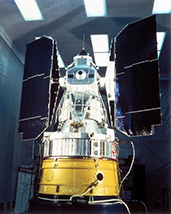
\includegraphics[totalheight=0.2\textheight]{Landsat1.jpg}
\caption{Landsat 1 (formerly named Earth Resources Technology Satellite ERTS-1) was launched on July 23, 1972. Photo Credits: \cite{landsat1}
}
\end{figure}

By the early 1980s, a second generation of instruments collecting satellite imagery provided far greater spatial resolution of 30, 20 and 10 meters. Eventually, by the late 1990s, images were capable of resolving at meter and  sub-meter levels \cite{campbell2011introduction}.

\par

%In summary, the Landsat constellation offered a way to observe the Earth in a repetitive and systematic way. It has contributed heavily to the understanding of Earth's environment, generated revolutionary uses of space-based data by the commercial sector and emboldened new generations of commercial and science satellites to provide high resolution spatial images of the entire Earth. \cite{campbell2011introduction, Williams:2006:0099-1112:1171}. 

As of September 1st 2021, there are 4,550 known operational satellites, of which 1030 are for Earth observation \cite{Sat_Data}. 

%This report will focus on cloud cover over Earth, weather forecasting and terrain identification

\subsection{EUMETSAT - Meteosat 9}


In this project, data from one of EUMETSAT's weather satellite Meteosat-9 is used. The satellite is jointly operated by the European Space Agency (ESA) and The European Organisation for the Exploitation of Meteorological Satellites (EUMETSAT). Meteosat-9 contains 12 spectral bands that covers the visible and infrared wavelengths. This project only uses three bands; one infrared and two visible bands. The satellite provides images over continental Africa every 15 minutes with a resolution of 5$\times$5 $\mathrm{~km}^{2}$ \cite{Meteosat9}. More information of Meteosat-9's twelve imaging bands are given in the Table 1 below.

\begin{table}[H]
\centering
\begin{tabular}{|l|l|}
\hline \textbf{Central wavelength} & \textbf{Spectral interval (99 \% encircled energy)} \\
\hline N/A (broad bandwidth channel) & $0.6-0.9 \mu \mathrm{m}$ \\
\hline $0.635 \mu \mathrm{m}$ & $0.56-0.71 \mu \mathrm{m}$ \\
\hline $0.81 \mu \mathrm{m}$ & $0.74-0.88 \mu \mathrm{m}$ \\
\hline $1.64 \mu \mathrm{m}$ & $1.50-1.78 \mu \mathrm{m}$ \\
\hline $3.92 \mu \mathrm{m}$ & $3.48-4.36 \mu \mathrm{m}$ \\
\hline $6.25 \mu \mathrm{m}$ & $5.35-7.15 \mu \mathrm{m}$ \\
\hline $7.35 \mu \mathrm{m}$ & $6.85-7.85 \mu \mathrm{m}$ \\
\hline $8.70 \mu \mathrm{m}$ & $8.30-9.10 \mu \mathrm{m}$ \\
\hline $9.66 \mu \mathrm{m}$ & $9.38-9.94 \mu \mathrm{m}$ \\
\hline $10.8 \mu \mathrm{m}$ & $9.80-11.8 \mu \mathrm{m}$ \\
\hline $12.0 \mu \mathrm{m}$ & $11.0-13.0 \mu \mathrm{m}$ \\
\hline $13.4 \mu \mathrm{m}$ & $12.4-14.4 \mu \mathrm{m}$ \\
\hline
\end{tabular}
\caption{\label{tab:Table1} Channel details of the Spinning Enhanced Visible Infra-Red Imager (SEVIRI). The instrument is sensitive to twelve channels (eleven narrow-bandwidth in the infrared and one high-resolution broad-bandwidth in the visible spectrum). Data from \cite{Table1}}
\end{table}



\subsection{Prior Work}\label{subsec1.3}

Solar power plants could have a very important role in the next decade. By forecasting short-term solar irradiation profiles, power plant operators are then able to make decisions on operating modes to optimise power output and use of storage systems such as large batteries, which promise reliability of storing renewable energy. Energy storage solutions as mentioned are able to balance the fluctuations in supply and demand and meet the growing demand for electricity \cite{joseph2006battery}. However, solar radiation can be blocked by cloud cover. Therefore, short term cloud forecasting can optimise power plant operation and therefore improve benefits and operational costs. Due to this, cloud detection, classification and motion vector determination are to key to accurate forecasts. Currently, Meteosat-9 is in geostationary orbit at an altitude of 36,000 km \cite{MS2G} observing continental Africa, whereby, Meteosat-9 can provide cloud information covering vast areas. This has the potential to give cloud forecasts several hours in advance so plant operation can improve by anticipating the power or battery storage use.
\par
Using Geosynchronous Meteorological Satellite-5 (GMS-5) cloud images were studied by \cite{janjai2009model} to create a model of calculating global solar radiation. The model represented a relation between earth-atmospheric albedo derived from GMS-5 satellite data and the absorption and scattering coefficients of various atmospheric constituents \cite{janjai2009model}.
\par
Further work has been done by \cite{globsol_NN} where Artificial Neural Networks (ANNs) have been used to estimate global solar radiation from Meteosat-9 data. The model's estimates are relativly accurate with spacially uniform errors. Even on cloudy days, the model yields reliable results. This has improved current models based on satellite imagery. \cite{janjai2009model}
\par
Meteosat data has been used for a variety of applications from cloud cover forecasting to maximise output of solar power plants \cite{cloud_forcast}, to determining cloud motion vectors \cite{cloudmotion} and estimating global solar radiation by using artificial neural networks \cite{globsol_NN}. 

\subsection{Project Aims}\label{subsec1.4}

Taking inspiration and account of the prior work that has been outlined in Section \ref{subsec1.3}, this project will aim to recreate RGB images from three separate greyscale images using the infrared (IR) and visible bands (VIS). Conjointly, we will attempt at cloud removal techniques. Lastly, we aim to measure the percentage change of cloud over over a period of time for a selected area of Earth.



